\documentclass[10pt]{article}
\usepackage{fullpage,enumitem,amsmath,amssymb,graphicx}
\usepackage{tikz}
\usepackage{array}
\usepackage{verbatim}

\begin{document}

\begin{center}
{\Large CS224N Winter 2016 Homework [3]}

\begin{tabular}{rl}
SUNet ID: & [jiajuns, xxx, xxx] \\
Name: & [Jiajun Sun, Sijun He, Mingxiang Chen] \\
\end{tabular}
\end{center}

By turning in this assignment, I agree by the Stanford honor code and declare
that all of this is my own work.

\section*{Problem 1}
\begin{enumerate}[label=(\alph*)]
\item
i.\\
Yesterday, price of Apple increased 6.56 percent.\\
Here apply can be interpreted as Apple company or the apple we eat.\\
\\
Mogen Stanley has bought a land besides Sand Hill Road as their bay area headquater.
Mogen Stanley can be interpreted as a name or a company.\\
\\

ii.\\
Words alone can have ambiguity, therefore adding features other than the word itself can help reduce ambiguity.\\
\\

iii.\\
First, the context of the word can help. The words around can imply the correct meaning of the center word.
Second, dependence structure could give the information on what is the function of the center word in the sentences.
This information can help interprete its entity.

\item
i.\\
$e^{(t)}$ has dimension of $1 \times 2(w+1)D$\\
$W$ has dimension of $2(w+1)D \times H$\\
$U$ has dimension of $H \times C$\\
\\
ii.\\
$$
\begin{aligned}
& cost(ReLu) = o(H) + o(2(w+1)D \times H)\\
& cost(softmax) = o(H \times C) + o(C)\\
& cost(CE) = o(C)
\end{aligned}
$$
Given the sentences has length of $T$, the computation complexity is:
$$
\begin{aligned}
cost
& = T \times o(o(H) + o(2(w+1)D \times H) + o(H \times C) + o(C) + o(C))\\
& \approx T o(2(w+1)D \times H)\\
& \approx T o(wDH)
\end{aligned}
$$

\item
(code)

\item
i.\\
Entity level P/R/F1: 0.82/0.84/0.83\\
\begin{table}[h]
	\centering
	\caption{confusion matrix}
	\begin{tabular}{|l|l|l|l|l|l|}
	\hline
	gogu & PER     & ORG     & LOC     & MISC    & O        \\ \hline
	PER   & 2940.00 & 56.00   & 46.00   & 13.00   & 94.00    \\ \hline
	ORG   & 128.00  & 1676.00 & 92.00   & 63.00   & 133.00   \\ \hline
	LOC   & 54.00   & 119.00  & 1845.00 & 29.00   & 47.00    \\ \hline
	MISC  & 36.00   & 63.00   & 35.00   & 1018.00 & 116.00   \\ \hline
	O     & 37.00   & 42.00   & 12.00   & 31.00   & 42637.00 \\ \hline
	\end{tabular}
\end{table}

ii.\\
First limitation is length of context is limited by the length of window size.
For example the \textbf{Test and County Cricket Board} does not get right label, because the length has exceeded the window size.\\
\\
Second limitation (some helps me out here)

\end{enumerate}

\begin{enumerate}[label=(\alph*)]
\item
i.\\
The number of RNN parameters:
$$
V \times D + H \times H + D \times H + H + H \times C + C
$$
The number of window-based model parameters:
$$
V \times D + D \times H + H + H \times C + C
$$
Therefore, RNN has $HH$ more parameters than window-based model.\\

ii.\\
Cost for one time step:
$$
\begin{aligned}
& cost(h) = o(H \times H) + o(D \times H) + o(H)\\
& cost(softmax) = o(H \times C) + o(C)\\
& cost(CE) = o(C)
\end{aligned}
$$
Adding them up:
$$
o(H \times H) + o(D \times H) + o(H) + o(H \times C) + o(C) + o(C) \approx o(H \times H) + o(D \times H)
$$
Therefore the total cost for sentence of length $T$:
$$
cost = T(o(H \times H) + o(D \times H))
$$

\item
i.\\
Consider a dataset that most of (over $90\%$) the entity is person,
if the model label all the entity as person the cross entropy error should be smaller.
However, by doing this the $F_1$ score should drop, because the prediction is biased and recall value will drop.

ii.\\
Optimizing $F_1$ score requires looking through the entire training set. The cost and memory requirement is huge.

\item
(code)

\item
The padded label $y$ will be transform into a one-hot vector.
When $y=0$, the corresponding one-hot vector is $[1, 0, 0, 0, 0]$.
Therefore, the padded label will be considered as label $o$.
The cross entropy loss is not always zero for the padded part.

\item
(code)

\item
result:

\item
explanation:

\end{enumerate}

\begin{enumerate}[label=(\alph*)]
\item
i.\\
$U_h = 1$, $W_h = 1$ and $b_h = 0$ will allow the RNN to replicate this behavior.\\

ii.\\
$U_z = 0$, $W_z = 1$, $U_h = 1$ and $W_h$ can be any value.\\
When $x=0$, $z_t = 0$ and $\tilde{h_t} = 0$ thus the hidden state will always be $h_t = 0$.
Whenever $x=1$, $z_t = 0$ and the hidden state will keep to be $h_t = h_{t-1} = 1$.

\item
i.\\
It is impossible for RNN to have togging behavior.
$U_t$ has to be a positive number in order to let $h_t$ switch to $1$.
Therefore for the second time when $x = 1$ it is impossible to let $h_t$ switch back to $0$.\\

ii.\\
$b_r = 1$, $U_z = -1$, $W_z = 1$, $U_h = 1$ and $W_h = -1$.
When $x=0$, $z_t = 0$ and $\tilde{h_t} = 0$ thus the hidden state will always be $h_t = 0$.
When $x=1$ for the first time, $z_t = 0$ but $\tilde{h_t} = 1$ thus the hidden state will switch to $h_t = 1$.
If $h_t=1$ and $x=0$, $z_t = 1$ and hidden state $h_t = h_{t-1} = 1$.
But if $x=1$, $z_t = 0$ and hidden state $h_t = \tilde{h_t} = 0$.

\item
(code)

\item
\begin{figure}[h]
\center
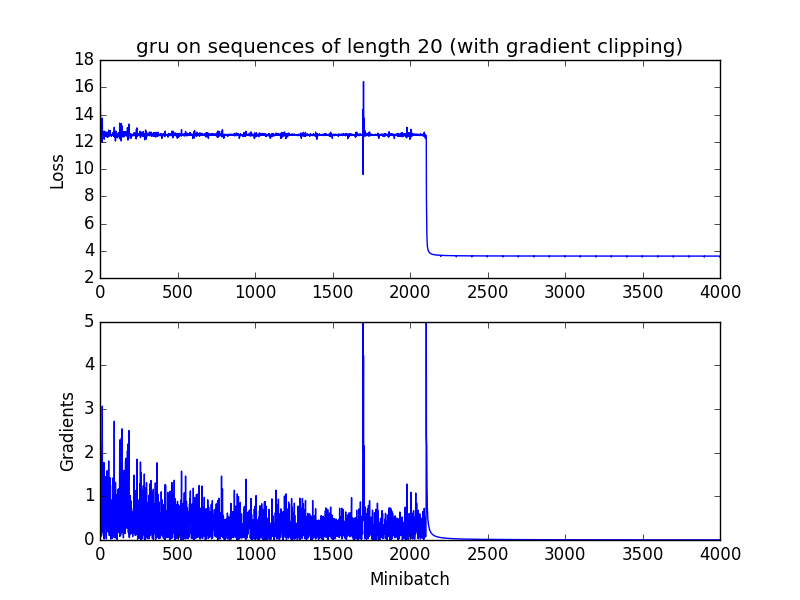
\includegraphics[scale=0.45]{q3-clip-gru.png}
\end{figure}

\begin{figure}[h]
\center
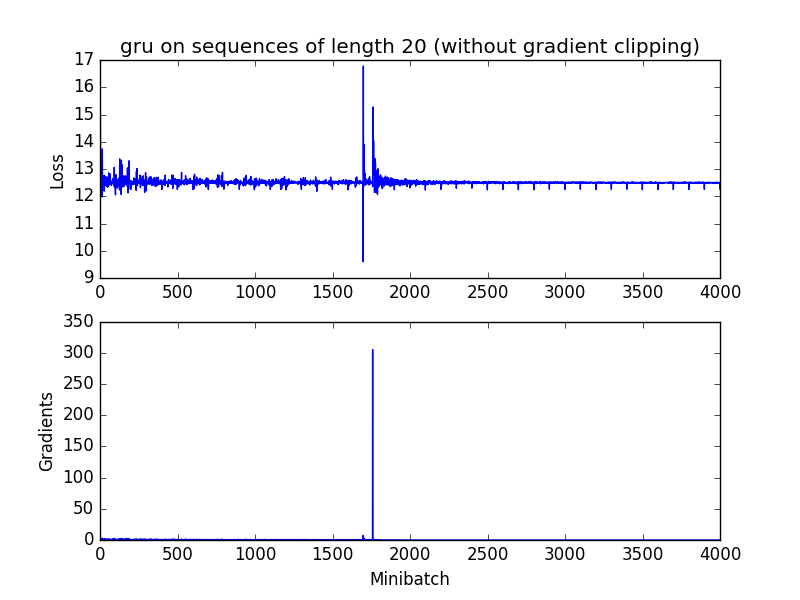
\includegraphics[scale=0.45]{q3-noclip-gru.png}
\end{figure}

\begin{figure}[h]
\center
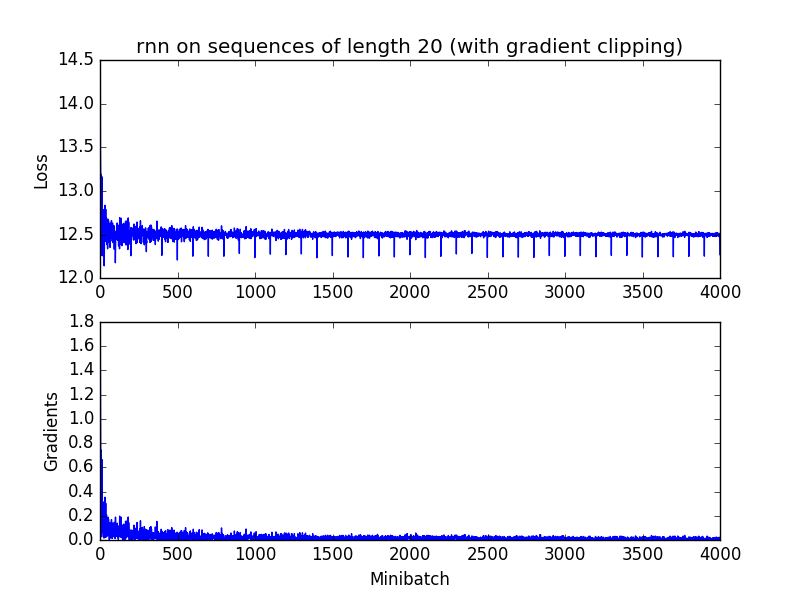
\includegraphics[scale=0.45]{q3-clip-rnn.png}
\end{figure}

\begin{figure}[h]
\center
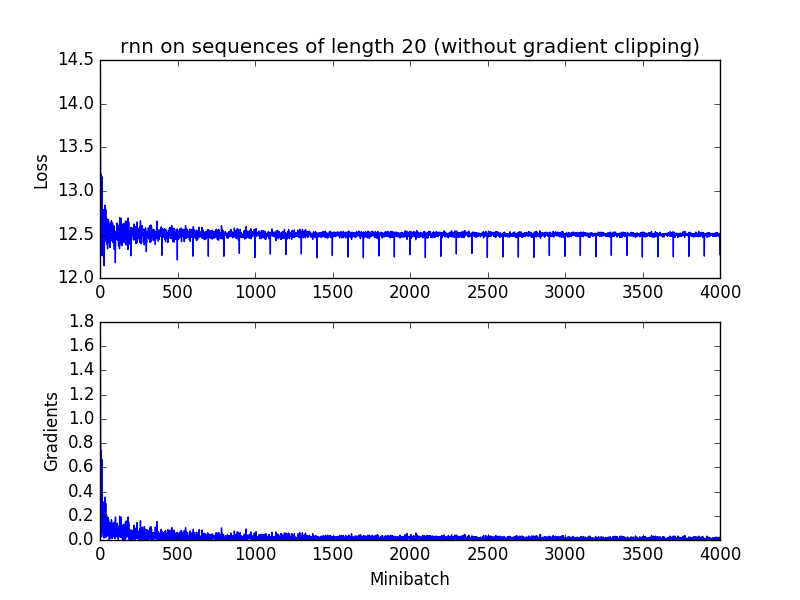
\includegraphics[scale=0.45]{q3-noclip-rnn.png}
\end{figure}

\item
explanation:

\item
waiting for the GPU then we can train this
F1 score


\end{enumerate}


\end{document}

